\documentclass[a4paper, 10pt]{article}
\usepackage[siunitx]{circuitikz}
\usepackage[margin=1in]{geometry}
\usepackage{subfiles}

\usetikzlibrary{intersections}

\begin{document}
\tikzset{blockdef-above/.style={%
	{Straight Barb[harpoon, right, length=-0.2cm]}-{Straight Barb[harpoon, left, length=-0.2cm]},
	black,
	}}

\tikzset{blockdef-below/.style={%
	{Straight Barb[harpoon, reversed, right, length=0.2cm]}-{Straight Barb[harpoon, reversed, left, length=0.2cm]},
	black,
	}}

\def\gateTransistor{$BC547$}
\def\baseResistor{\SI{220}{k\ohm}}
\def\outResistor{\SI{47}{k\ohm}}
\def\ledResistor{\SI{18}{k\ohm}}
\def\vccPotential{$V_{CC}=\SI{5}{V}$}

\clearpage

\section{Logic Gates}

\subsection{AND Gate}

\begin{figure}[!ht]
	\centering
    \includegraphics{tikzpics/epictlvlandgate.pdf}
	\caption{\textbf{AND} Gate}
\end{figure}

\subsection{OR Gate}

\begin{figure}[!hb]
	\centering
    \includegraphics{tikzpics/epictlvlorgate.pdf}
	\caption{\textbf{OR} Gate}
\end{figure}

\subsection{XOR Gate}

\begin{figure}[!hp]
	\centering
    \includegraphics{tikzpics/epictlvlxorgate.pdf}
	\caption{\textbf{XOR} Gate}
\end{figure}

\clearpage

\section{Adders}

\subsection{Half Adder}

\begin{figure}[!ht]
	\centering
    \includegraphics{tikzpics/epicglvlhalfadder.pdf}
	\caption{Half Adder}
\end{figure}

\vspace{0.2\textheight}

\subsection{Full Adder}

\begin{figure}[!hb]
	\centering
    \includegraphics{tikzpics/epicglvlfulladder.pdf}
	\caption{Full Adder}
\end{figure}

\clearpage

\subsection{Full Adder from Raw \textbf{Transistors}}

\begin{figure}[!h]
	\centering
	\resizebox{\textwidth}{!}{
    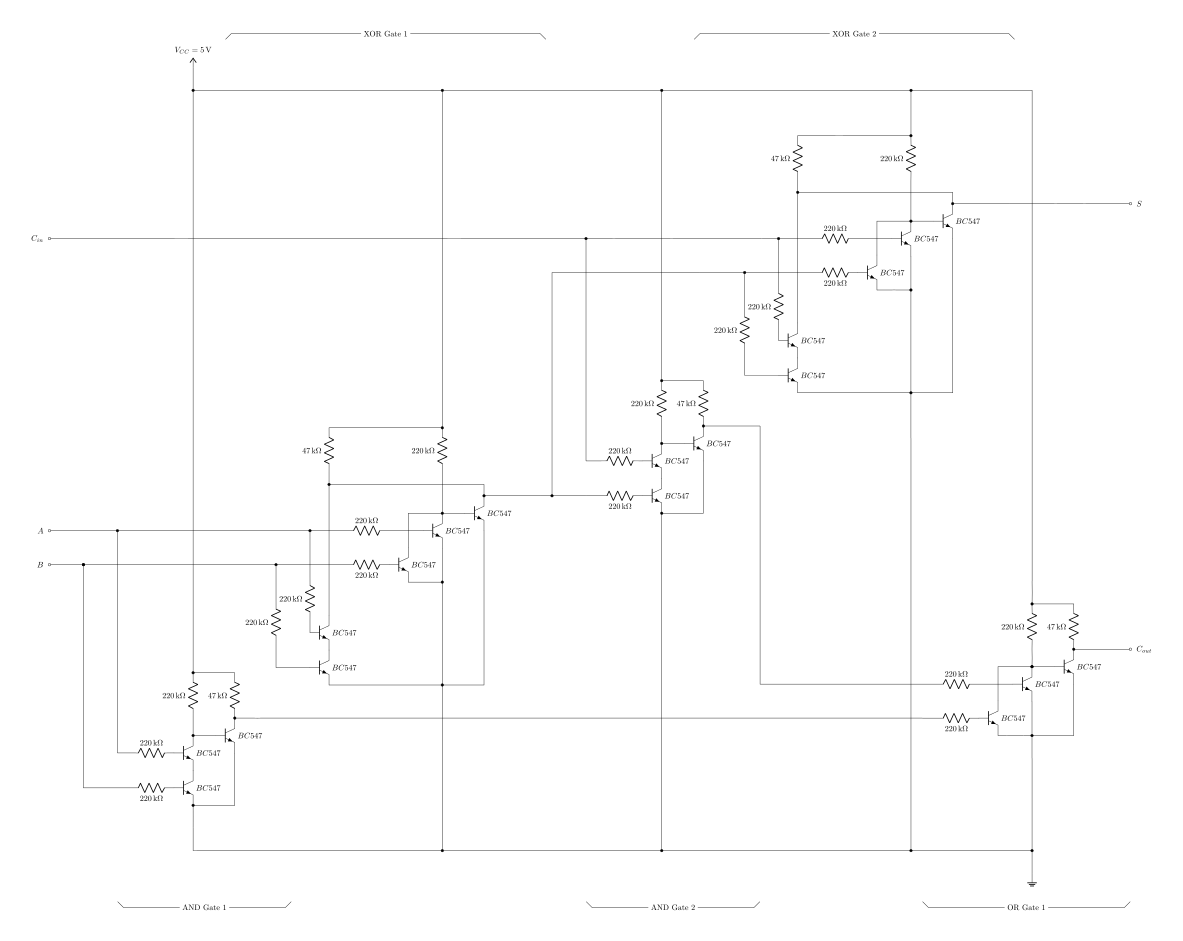
\includegraphics{tikzpics/epictlvlfulladder.pdf}
	}
	\caption{Full Adder from Raw \textbf{Transistors}}
\end{figure}

\clearpage

\section{Control Unit}

\subsection{Control Unit for 4 bit Ripple Adder}

\begin{figure}[!h]
    \centering
    \resizebox{!}{0.8\textheight}{
        \includegraphics{tikzpics/epicfourbitaddercu.pdf}
    }
    \caption{Control Unit for \textbf{4 bit Ripple Adder}}
\end{figure}


\clearpage

\subsection{Control Unit for Full Adder}

\begin{figure}[!h]
	\centering
	\resizebox{\textwidth}{!}{
		\begin{tikzpicture}[american]

		\draw (0,0)
		node (S1) [spdt] {}

		(S1.in) to[short, -*] ++(-0.5,0)
		coordinate (S1br)
		to[short, -o] ++(-2,0)
		coordinate (A)
		node [left=4pt] {$A$}

		(S1br) -- ++(0,-0.5)
		to[R, l=\ledResistor] ++(0,-2)
		to[leDo] ++(0,-2)
		-- ++(0,-0.5)
		coordinate (Gbr)

		(S1.out 2) -- ++(0.5,0)
		coordinate (S1outbr)
		to[short, -*] (S1outbr|-Gbr)

		(S1.out 1) -- (S1.out 1-|S1outbr)
		to[short, -*] ++($(S1.out 2)-(S1.out 2|-Gbr)$)
		coordinate (Vbr)

		(S1.out 1) ++(4.5,1)
		node (S2) [spdt, anchor=out 1] {}
		(S2.out 1) -- ++(0.5,0)
		coordinate (S2outbr)

		to[short, -*] (S2outbr|-Vbr)
		(S2.out 2) -- (S2outbr|-S2.out 2)
		to[short, -*] (S2outbr|-Gbr)

		(S2.in) to[short, -*] ++(-0.5,0)
		coordinate (S2br)
		to[short, -o] (S2br-|A)
		coordinate (B)
		node [left=4pt] {$B$}

		(S2br) to[R, l=\ledResistor] ++(0,-2)
		to[leDo] ++(0,-2)
		to[short, -*] (S2br|-Gbr)

		(S2.out 1) ++(4.5,1)
		node (S3) [spdt, anchor=out 1] {}
		(S3.out 1) -- ++(0.5,0)
		coordinate (S3outbr)

		to[short, -*] (S3outbr|-Vbr)
		(S3.out 2) -- (S3outbr|-S3.out 2)
		to[short, -*] (S3outbr|-Gbr)

		(S3.in) to[short, -*] ++(-0.5,0)
		coordinate (S3br)
		to[short, -o] (S3br-|A)
		coordinate (Cin)
		node [left=4pt] {$C_{in}$}

		(S3br) to[R, l=\ledResistor] ++(0,-2)
		to[leDo] ++(0,-2)
		to[short, -*] (S3br|-Gbr)

		(S1.in-|S3.in) ++(4,0)
		node (nb1) [npn, xscale=-1, anchor=C] {
			\scalebox{-1}[1]{\gateTransistor}}

		(nb1.C) -- ++(0,-0.5)
		to[leDo, invert, mirror] ++(0,2)
		to[R, l=\ledResistor] ++(0,2)
		to[short, -*] (nb1.C|-Vbr)

		(nb1.E) to[short, -*] (nb1.E|-Gbr)

		(nb1.B) -- ++(2.25,0)
		to[R, l=\baseResistor] ++(2,0)
		to[short, -o] ++(0.5,0)
		coordinate (S)
		node [right=4pt] {$S$}

		(nb1.C) ++(2.25,1)
		node (nb2) [npn, xscale=-1, anchor=C] {
			\scalebox{-1}[1]{\gateTransistor}}

		(nb2.C) -- ++(0,-0.5)
		to[leDo, invert, mirror] ++(0,2)
		to[R, l=\ledResistor] ++(0,2)
		-- (nb2.C|-Vbr)

		(nb2.E) to[short, -*] (nb2.E|-Gbr)

		(nb2.B) to[R, l=\baseResistor] ++(2,0)
		to[short, -o] (nb2.B-|S)
		coordinate (Cout)
		node [right=4pt] {$C_{out}$}

		(Cin) ++($(Cin)-(B)$)
		coordinate (Vout)
		node [left=4pt] {$V_{out}$}
		to[short, o-*] (Vout-|S3outbr)

		(S) ++($(S)-(Cout)$)
		coordinate (Gout)
		node [right=4pt] {$G_{out}$}
		to[short, o-*] (Gout-|S3outbr)

		(nb2.C|-Vbr) -- (S1outbr|-Vbr)
		-- ++(0,1.5)
		coordinate (V)
		node [vcc] {\vccPotential}

		(S1br|-Gbr) -- (nb2.E|-Gbr)
		-- ++(0,-1.5)
		coordinate (G)
		node [ground] {}

		;

	\end{tikzpicture}
	}
	\caption{Control Unit for \textbf{Full Adder}}
\end{figure}

\end{document}
